\documentclass[aspectratio=169]{beamer}
\usepackage[T1]{fontenc}
\usepackage[english]{babel}
\usetheme{Madrid}
\usecolortheme{default}
% \usepackage[utf8]{vietnam}
\usepackage{amsmath, amssymb, amsfonts}
\usepackage{algorithm}
\usepackage[noend]{algpseudocode}
\usepackage{svg}
\beamertemplatenavigationsymbolsempty
\usepackage[backend=biber, defernumbers=true,style=authortitle-ibid,citetracker=true,maxnames=1, minnames=1,sorting=none,doi=false,url=false]{biblatex}

\DefineBibliographyStrings{english}{%
    andothers={et al.},
}

\addbibresource{bitex/ThOP.bib}
\addbibresource{bitex/ACOThOP.bib}
\addbibresource{bitex/ACO++ThOP.bib}
\addbibresource{bitex/AACONC.bib}
\addbibresource{bitex/ACO.bib}
\addbibresource{bitex/CMA-ES.bib}

\title[Thief Orienteering Problem]
{Investigating the Orienteering Problem with a capacity constraint}

\author[Viet Le, Vu Huynh]{
    \begin{columns}[T]
        \column{.28\textwidth}
            \centering
            \usebeamerfont{author}Viet Le\\
                20520093@gm.uit.edu.vn
        \column{.25\textwidth}
            \centering
            \usebeamerfont{author}Vu Hoang Huynh\\
                20520864@gm.uit.edu.vn
    \end{columns}
}
\institute[UIT]
{
    Vietnam National University, Ho Chi Minh City - University of Information Technology
    \\ \vspace{1cm}
    \large Subject: Specialized Project
    \\ \vspace{0.5cm}
    Instructor: PhD. Ngoc Hoang Luong
}

\date[July 2023]
{July 2023}

\AtBeginSection[]
{
  \begin{frame}
    \frametitle{Table of Contents}
    \tableofcontents[currentsection]
  \end{frame}
}


\begin{document}

\frame{\titlepage}

\begin{frame}
        \frametitle{Table of Contents}
        \tableofcontents[2]
\end{frame}

\section{Introduction}
\subsection{Problem description}
\begin{frame}{Problem description}
    % \hspace{0.1cm}
        \vspace*{-0.25cm}
            \begin{block}{Thief orienteering problem (ThOP)}
                \footnotesize ThOP\footnotemark is a \textbf{multi-component optimization problem}, it combines the \textbf{Orienteering Problem (OP)} and \textbf{Knapsack Problem (KP)}.
            \end{block}
    \footnotetext{\fullcite{Santos2018TheTO}}
\end{frame}

\begin{frame}{Problem description}
    % \hspace{0.1cm}
        \onslide<1->{
            \begin{columns}
                \hspace{0.17cm}\begin{column}{0.55\textwidth}
                    \begin{block}{Orienteering problem (OP)}
                         \footnotesize OP is a \textbf{routing problem} in which the goal is to determine a path through a given set of points of interest that \textbf{maximizes a total score} while \textbf{satisfying a given time budget}.
                    \end{block}
                \end{column}
                
                \begin{column}{0.45\textwidth}
                    \begin{center}
                        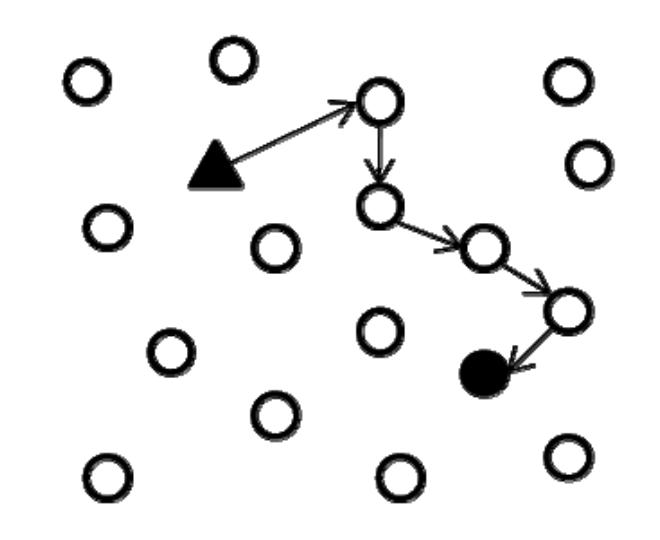
\includegraphics[scale=0.25]{img/orienteering.jpg}
                    \end{center}
                \end{column}
            \end{columns}
        }
        \onslide<2->{
            \begin{columns}
                \hspace{0.17cm}\begin{column}{0.55\textwidth}
                     \begin{block}{Knapsack problem (KP)}
                        \footnotesize KP is an \textbf{optimization problem} in which the goal is to \textbf{select a subset of items} from a given set such that \textbf{the total value} of the selected items \textbf{is maximized}, while the \textbf{total weight} of the selected items does \textbf{not exceed a given capacity}.
                    \end{block}
                \end{column}
                
                \begin{column}{0.45\textwidth}
                    \begin{center}
                        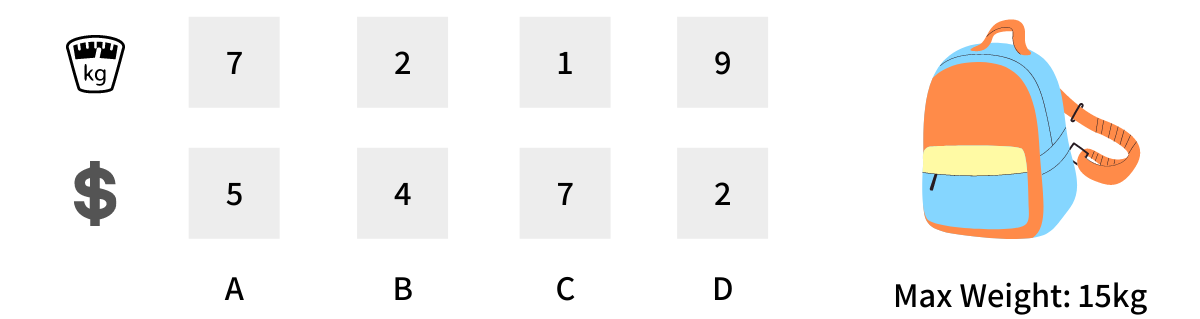
\includegraphics[scale=0.15]{img/knapsack.png}
                    \end{center}
                \end{column}
            \end{columns}   
        }
        
\end{frame}

\subsection{Example}
\begin{frame}{Example}
    \begin{columns}
        \begin{column}{0.5\textwidth}
            \begin{center}
                \only<1>{
                \includesvg[inkscapelatex=false,width=\columnwidth]{img/Example1.svg}
                }
                \only<2>{
                \includesvg[inkscapelatex=false,width=\columnwidth]{img/Example2.svg}
                }
                \only<3>{
                \includesvg[inkscapelatex=false,width=\columnwidth]{img/Example3.svg}
                }
                \only<4>{
                \includesvg[inkscapelatex=false,width=\columnwidth]{img/Example4.svg}
                }
            \end{center}   
            
        \end{column}
        
        \begin{column}{0.45\textwidth}
            \only<1>{
                \vspace{-5cm}
                \begin{block}{\small Constraints}
                    \footnotesize
                    \begin{itemize}
                    \item $n = 4, m = 5$
                    \item $v_{min} = 0.1, v_{max}  = 1.0, W = 3, T = 75$
                    \end{itemize}
                    
                \end{block}
            }
            \only<2>{
            
                \begin{block}{\small Constraints}
                    \footnotesize
                    \begin{itemize}
                    \item $n = 4, m = 5$
                    \item $v_{min} = 0.1, v_{max}  = 1.0, W = 3, T = 75$
                    \end{itemize}
                    
                \end{block}
                \begin{block}{\small Solution}
                    \footnotesize
                    \begin{itemize}
                    \item $\pi = \langle 1 \rangle\⟩$
                    \item $p = \langle0, 0, 0 ,0 ,0\rangle$
                    \end{itemize}    
                \end{block}
                
                \begin{block}{\small Properties}
                    \footnotesize
                    \begin{itemize}
                    \item $p = 0$
                    \item $w = 0$
                    \item $v = v_{max} = 1.0$
                    \item $t = 0$
                    \end{itemize}
                    
                \end{block}
            }

            \only<3>{
            
                \begin{block}{\small Constraints}
                    \footnotesize
                    \begin{itemize}
                    \item $n = 4, m = 5$
                    \item $v_{min} = 0.1, v_{max}  = 1.0, W = 3, T = 75$
                    \end{itemize}
                    
                \end{block}
                \begin{block}{\small Solution}
                    \footnotesize
                    \begin{itemize}
                    \item $\pi = \langle 1, 3 \rangle\⟩$
                    \item $p = \langle0, 0, 0 ,0 ,0\rangle$
                    \end{itemize}    
                \end{block}
                
                \begin{block}{\small Properties}
                    \footnotesize
                    \begin{itemize}
                    \item $p = 0$
                    \item $w = 0$
                    \item $v = v_{max} = 1.0$
                    \pause
                    \item $t = d_{1,3} / v = 6 / 1.0 = 6$
                    \end{itemize}
                    
                \end{block}
            }

            \only<4>{
            
                \begin{block}{\small Constrains}
                    \footnotesize
                    \begin{itemize}
                    \item $n = 4, m = 5$
                    \item $v_{min} = 0.1, v_{max}  = 1.0, W = 3, T = 75$
                    \end{itemize}
                    
                \end{block}
                \begin{block}{\small Solution}
                    \footnotesize
                    \begin{itemize}
                    \item $\pi = \langle 1, 3, 4 \rangle\⟩$
                    \item $p = \langle0, 0, 1 ,0 ,0\rangle$
                    \end{itemize}    
                \end{block}
                
                \begin{block}{\small Properties}
                    \footnotesize
                    \begin{itemize}
                    \item $p = 100$
                    \item $w = 0 + w_{3} = 3$
                    \pause
                    \item $v = v_{max} - w (v_{max} - v_{min}) / W = 0.1$
                    \pause
                    \item $t = t + d_{3,4} / v = 6 + 5 / 0.1 = 56$
                    \end{itemize}
                    
                \end{block}
            }
        \end{column}
    \end{columns}
\end{frame}

\subsection{Motivation}
\begin{frame}{Motivation}
    \begin{block}{Theoretical Motivation}
        \vspace{0.2cm}
        \begin{itemize}
            \item ThOP can be a benchmark for evaluating and comparing optimization methods.
            \item ThOP can contribute to solving its component problems OP and KP, even TTP and TSP.
        \end{itemize}
        \vspace{0.2cm}
    \end{block}
    \pause
    \begin{block}{Practical Motivation}
        \vspace{0.2cm}
        ThOP can be generalized to solve real-world problems:
        \begin{itemize}
            \item Planing a route for a vehicle to collect packages in multiple warehouses with time constraints and capacity limits.
            \item Planing a route for a rescue team to visit a set of locations to collect supplies and rescue victims.
        \end{itemize}
        \vspace{0.2cm}
    \end{block}
\end{frame}

\section{The State-Of-The-Art}
\subsection{Background}
\begin{frame}{Background}
\begin{itemize}
    \item Ant Colony Optimization (ACO)\footnotemark
    
    \footnotetext{\fullcite{4129846}}
    \vspace{0.2cm}
    \item ACO for ThOP\footnotemark
    \vspace{0.2cm}
    \item Randomized Packing Heuristic\footnote[3]

    \footnotetext{\fullcite{Chagas2020}}
\end{itemize}
\end{frame}
\begin{frame}{Ant Colony Optimization}
\begin{columns}
    \hspace{0.1cm}
    \begin{column}{0.25\textwidth}
        \includesvg[inkscapelatex=false,width=\columnwidth]{img/ACO original.svg}
    \end{column}
    
    \begin{column}{0.75\textwidth}  
    \begin{center}
    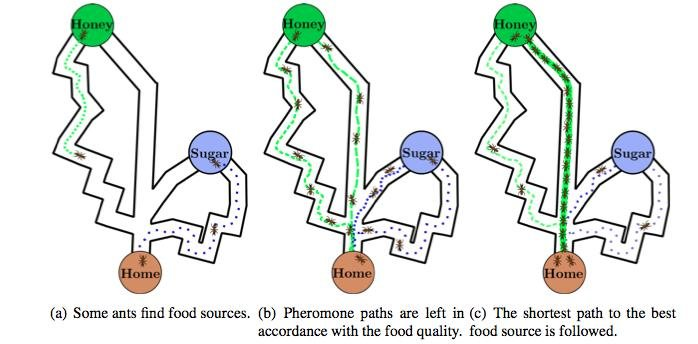
\includegraphics[scale=0.6]{img/The-concept-of-ant-colony-optimization.jpg}
    \end{center}
    \end{column}
\end{columns}
\end{frame}

% \begin{frame}{ACO for ThOP}
% \vspace*{-0.3cm}
% \begin{columns}
%     \begin{column}{0.5\textwidth}
%     \begin{center}
%         \includesvg[inkscapelatex=false,width=0.55\columnwidth]{img/ACO original 2.svg} 
%     \end{center}
%     \end{column}
    
%     \begin{column}{0.5\textwidth}  
%     \begin{center}
%         \includesvg[inkscapelatex=false,width=0.68\columnwidth]{img/ACO for ThOP.svg}
%     \end{center}
%     \end{column}
% \end{columns}
% \begin{columns}
%     \begin{column}{0.5\textwidth}
%     \begin{center}
%         \scriptsize \textbf{ACO} \\
%     \end{center}
%     \end{column}
    
%     \begin{column}{0.5\textwidth}  
%     \begin{center}
%         \scriptsize \textbf{ACO for ThOP} \\
%     \end{center}
%     \end{column}
% \end{columns}
% \end{frame}

\begin{frame}{ACO for ThOP}
\vspace{0.1cm}
\centering
\includesvg[inkscapelatex=false,width=0.9\columnwidth]{img/ACO for ThOP_Dashed Line.svg}
\end{frame}

\begin{frame}{Randomized Packing Heuristic}
\begin{block}{Score}
\vspace{0.2cm}
For each item $i$, there is a score $s_i$ that takes into account a trade-off between the distance that the item needs to be transported, its weight, and its profit.
\vspace{0.2cm}
$$s_i = {p_i^\theta \over w_i^\delta * d_i^\gamma}$$
\vspace{0.2cm}
\end{block}
\end{frame}

\begin{frame}{Randomized Packing Heuristic}
$$s_i = {p_i^\theta \over w_i^\delta * d_i^\gamma}$$
\begin{block}{Description}
\begin{itemize}
\vspace{0.2cm}
    \item $p_i$ is the profit of item $i$
\vspace{0.2cm}
    \item $w_i$ is the weight of item $i$
\vspace{0.2cm}
    \item $d_i$ is the distance from the city containing item $i$ to the ending city according to the route
\vspace{0.2cm}
    \item $\theta$, $\delta$, $\gamma$ in range $[0, 1]$
\end{itemize}
\vspace{0.2cm}
\end{block}
\end{frame}

\begin{frame}{Randomized Packing Heuristic}

\begin{block}{Pseudocode}
    \begin{enumerate}
        \vspace{0.2cm}
        \item Generate random number $\theta$, $\delta$ and $\gamma$ in the range $[0, 1]$
        \pause
        \vspace{0.2cm}
        \item Normalize $\theta$, $\delta$, $\gamma$ such that $\theta + \delta + \gamma = 1$
        \pause
        \vspace{0.2cm}
        \item For each item $i$, compute score $s_i$
        \pause
        \vspace{0.2cm}
        \item While not violating constraints, pick an item having next highest score
        \pause
        \vspace{0.2cm}
        \item Repeat all steps above max\_packing\_tries times
        \vspace{0.2cm}
        \item Return the packing plan having best profit
        \vspace{0.2cm}
    \end{enumerate}
\end{block}
\end{frame}

\subsection{ACO++}
\begin{frame}{ACO++}
\begin{block}{}
\begin{itemize}
    \vspace{0.2cm}
    \item ACO++\footnotemark  algorithm is a combination of a heuristic approach based on Ant Colony Optimization with a randomized packing heuristic and with local searches.
    \vspace{0.2cm}
    \item ACO++ outperformed all other algorithms (ACO, BRKGA, ILS, GA) by more than 96\% of the total of test cases.\footnotemark[4]
    \vspace{0.2cm}
\end{itemize}
\end{block}
\footnotetext{\fullcite{Chagas2021}}
\end{frame}

\begin{frame}{ACO++}
\vspace*{-0.2cm}
\begin{columns}
    \begin{column}{0.5\textwidth}
    \begin{center}
        \includesvg[inkscapelatex=false,width=0.55\columnwidth]{img/ACO for ThOP 2.svg}
    \end{center}
    \end{column}
    
    \begin{column}{0.5\textwidth}  
    \begin{center}
        \includesvg[inkscapelatex=false,width=0.55\columnwidth]{img/ACO++.svg} 
    \end{center}
    \end{column}
\end{columns}
\begin{columns}
    \begin{column}{0.5\textwidth}
    \begin{center}
        \scriptsize \textbf{ACO for ThOP} \\
    \end{center}
    \end{column}
    
    \begin{column}{0.5\textwidth}  
    \begin{center}
        \scriptsize \textbf{ACO++} \\
    \end{center}
    \end{column}
\end{columns}
\end{frame}

\begin{frame}{ACO++ - Drawbacks}
\begin{itemize}
    \item The packing algorithm relies heavily on randomness.
\end{itemize}
\begin{block} {Packing Algorithm}
\begin{enumerate}
    \vspace{0.2cm}
    \color{red}
    \item \textbf{Generate random number $\theta$, $\delta$ and $\gamma$ in the range $[0, 1]$}
    \color{black}
    \vspace{0.2cm}
    \item Normalize $\theta$, $\delta$, $\gamma$ such that $\theta + \delta + \gamma = 1$
    \vspace{0.2cm}
    \item For each item $i$, compute score $s_i$
    \vspace{0.2cm}
    \item While not violating constraints, pick an item having next highest score
    \vspace{0.2cm}
    \item Repeat all steps above max\_packing\_tries times
    \vspace{0.2cm}
    \item Return the packing plan having best profit
    \vspace{0.2cm}
\end{enumerate}
\end{block}
\end{frame}

\begin{frame}{ACO++ - Drawbacks}
\begin{itemize}
    \item The hyperparameters are sensitive.
\end{itemize}
\begin{columns}
    \column{.5\textwidth}
    \centering
    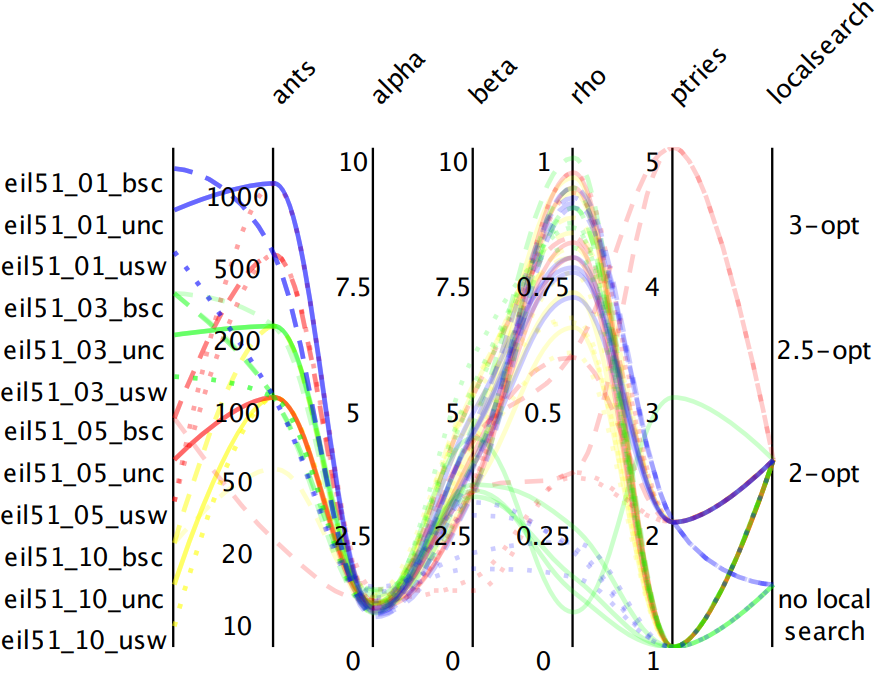
\includegraphics[scale=0.45]{img/eil51.png}
    
    \column{.5\textwidth}
    \centering
    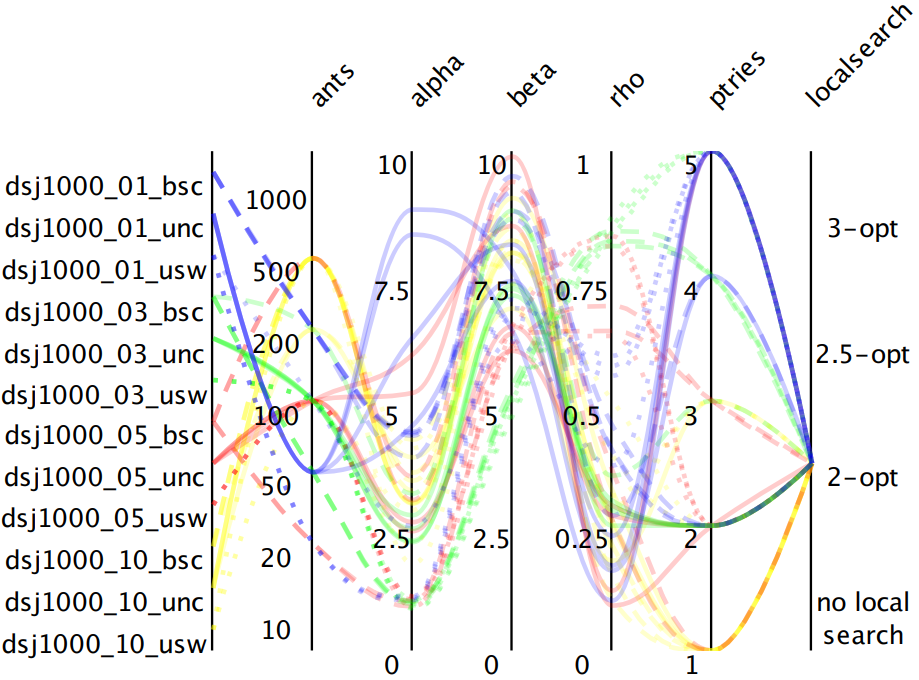
\includegraphics[scale=0.45]{img/dsj1000.png}        
\end{columns}
\end{frame}

\section{Our Experiment}
% \subsection{AACO-NC Experiment}

% \begin{frame}{AACO-NC}
%     \begin{block}{Adaptive Ant Colony Optimization with Node Clustering}
%     AACO-NC\footnotemark is a \textbf{metaheuristic algorithm} based on the Ant Colony Optimization (ACO) theory that is proposed to \textbf{solve the TSP}. This algorithm uses 2 primary mechanisms: \textbf{Adaptive pheromone evaporation} and \textbf{Node Clustering}.
%     \end{block}
%     \begin{block}{Adaptive pheromone evaporation}
%     \begin{itemize}
%         \item Using entropy information of the current set of solutions of the ant colony to adjust pheromone evaporation rate.
%         \item When the current population has \textbf{high entropy} the algorithm then \textbf{increases the evaporation rate}, otherwise \textbf{reducing the evaporation rate}.
%     \end{itemize}
    
%     \end{block}
%     \footnotetext{\fullcite{STODOLA2022101056}}
% \end{frame}

% \begin{frame}{AACO-NC}
%     \begin{block}{Node Clustering}
%     Using the node clustering principle instead of nearest neighbors when choosing the next potential city candidates.
%     \end{block}
    
%    \begin{center}
%        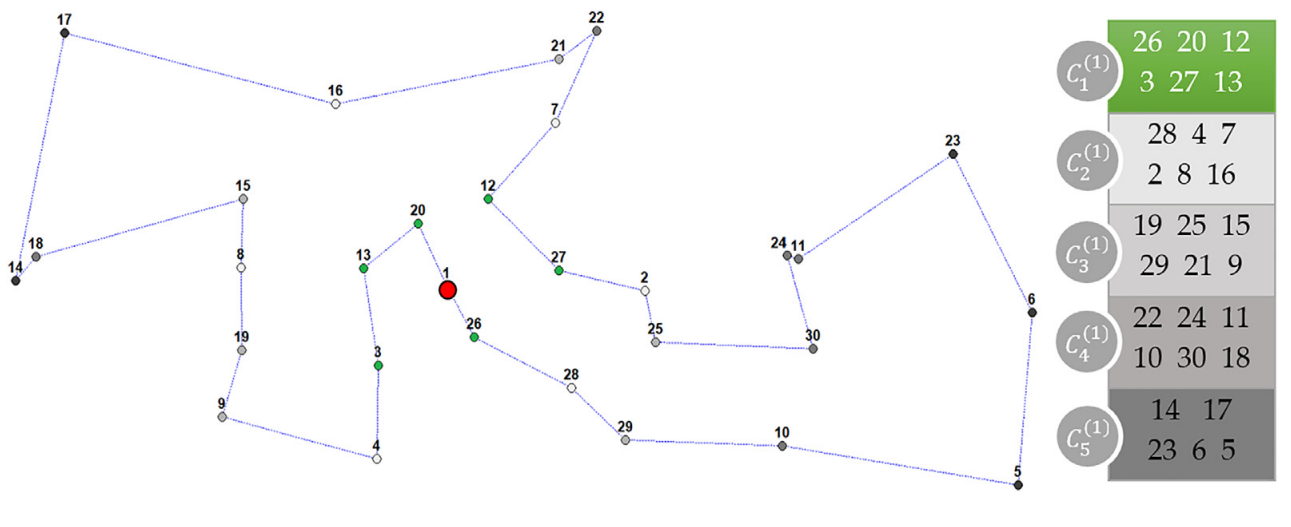
\includegraphics[scale=0.4]{img/nodeclustering.png}
%    \end{center}
% \end{frame}

% \begin{frame}{AACO-NC}
% \centering
% \includesvg[inkscapelatex=false,width=0.3\columnwidth]{img/ACO++ 3.svg}
% \\ \scriptsize \textbf{ACO++}
% \end{frame}

% \begin{frame}{AACO-NC Experiment}
% \begin{block} {Result}
% \begin{itemize}
%     \vspace{0.2cm}
%     \item Do experiment on \textbf{108} test cases.
%     \vspace{0.2cm}
%     \item \textbf{8.33\%} of test cases, \textbf{AACO-NC} is \textbf{better} \textbf{0.27\%} on profit on average.
%     \vspace{0.2cm}
%     \item \textbf{91.67\%} of test cases, \textbf{ACO++} is \textbf{better} \textbf{4.36\%} on profit on average.
%     \vspace{0.2cm}
% \end{itemize}
% \end{block}
% \end{frame}


% \subsection{CMA-ES Experiment}
\begin{frame}{CMA-ES}
\begin{columns}
\hspace{0.2cm}
\column{0.5\textwidth}
\begin{block} {Introduction}
\vspace{0.2cm}
CMA-ES\footnotemark stands for \textbf{Covariance Matrix Adaptation Evolution Strategy}, which is a \textbf{stochastic}, \textbf{derivative-free} method for numerical optimization of \textbf{non-linear} or \textbf{non-convex} \textbf{continuous} optimization problems. \\
\vspace{0.2cm}
\end{block}
\column{0.5\textwidth}
\centering
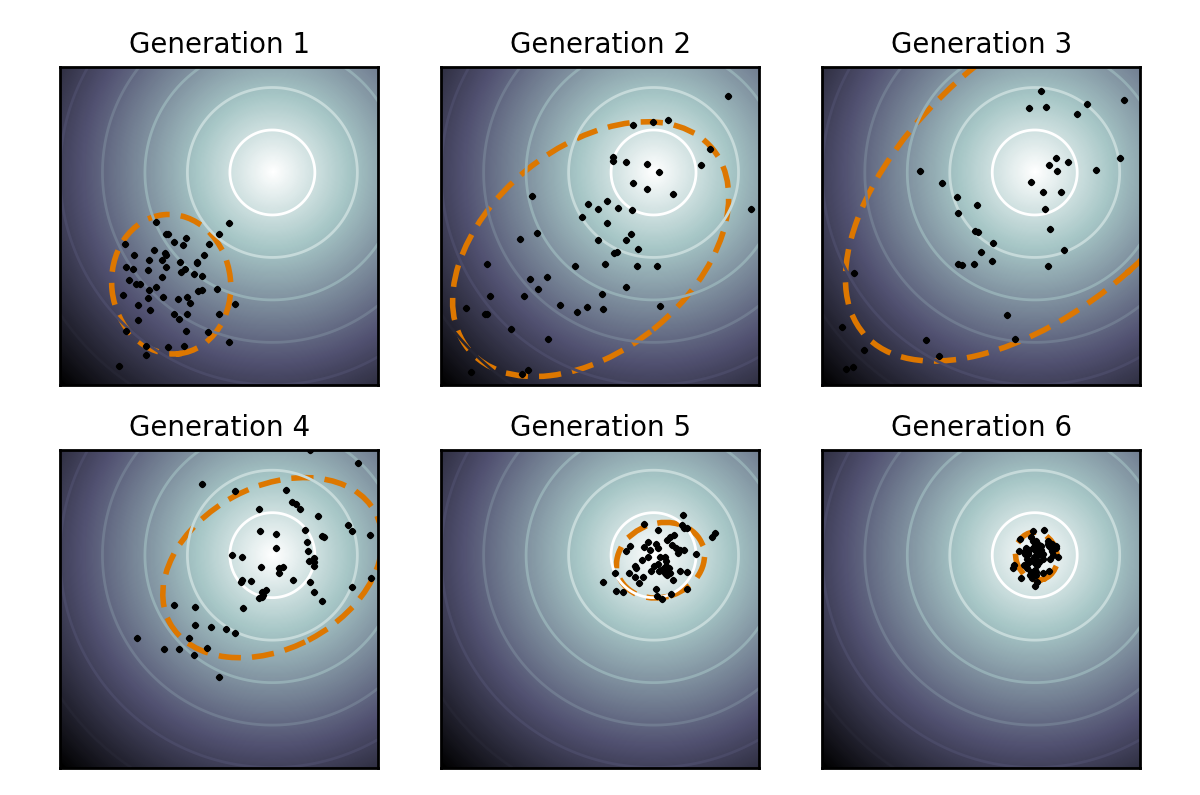
\includegraphics[scale=0.5]{img/CMA-ES.png}
    
\end{columns}
\footnotetext{\fullcite{Hansen2001}}
\end{frame}

% \begin{frame}{CMA-ES Experiment}
% \vspace*{-0.2cm}
% \begin{columns}
%     \begin{column}{0.5\textwidth}
%     \begin{center}
%         \includesvg[inkscapelatex=false,width=0.55\columnwidth]{img/ACO++ 2.svg}
%     \end{center}
%     \end{column}
    
%     \begin{column}{0.5\textwidth}  
%     \begin{center}
%         \includesvg[inkscapelatex=false,width=0.55\columnwidth]{img/CMA-ES.svg} 
%     \end{center}
%     \end{column}
% \end{columns}
% \begin{columns}
%     \begin{column}{0.5\textwidth}
%     \begin{center}
%         \scriptsize \textbf{ACO++} \\
%     \end{center}
%     \end{column}
    
%     \begin{column}{0.5\textwidth}  
%     \begin{center}
%         \scriptsize \textbf{Our Proposed Algorithm} \\
%     \end{center}
%     \end{column}
% \end{columns}
% \end{frame}

\begin{frame}{Experiment - Our proposed method}
\vspace{0.15cm}
\centering
\includesvg[inkscapelatex=false,width=0.8\columnwidth]{img/CMA-ES_Dashed Line.svg}
\end{frame}

\begin{frame}{Experiment - Our proposed method}
\begin{block} {}
\begin{itemize}
    \vspace{0.2cm}
    \vspace{0.2cm}
    \item Adaptation Mechanism from AACO-NC\footnotemark
    \vspace{0.2cm}
    \item Hierarchical Clustering
    \vspace{0.2cm}
\end{itemize}
\end{block}
    \footnotetext{\fullcite{STODOLA2022101056}}
\end{frame}


\begin{frame}{Experiment - Result}
\begin{block} {Result}
\begin{itemize}
    \vspace{0.2cm}
    \item \color{red} \textbf{59.03\%} \color{black} of test cases, \color{red} \textbf{our proposed algorithm} \color{black} is \color{red} \textbf{better} \textbf{1.11\%} \color{black} on profit on average.
    \vspace{0.2cm}
    \item \textbf{40.97\%} of test cases, \textbf{ACO++} is \textbf{better} \textbf{1.29\%} on profit on average.
    \vspace{0.2cm}
\end{itemize}
\end{block}
\end{frame}

\section{Future Works}
\begin{frame}{Future Works}
\begin{block} {}
\begin{itemize}
    \vspace{0.2cm}
    \item Run the experiment with more random seed.
    \pause
    \vspace{0.2cm}
    \item Utilize crossover operations in the genetic algorithms during the local search phase.
    \pause
    \vspace{0.2cm}
    \item Improve packing strategy.
    \vspace{0.2cm}
\end{itemize}
\end{block}
\end{frame}

\begin{frame}
\begin{center}
    \Huge \texttt{Thank you for listening}
\end{center}
\end{frame}

\begin{frame}{References}
\text{[1]} \fullcite{Santos2018TheTO}\\
\text{[2]} \fullcite{4129846}\\
\text{[3]} \fullcite{Chagas2020}\\
\text{[4]} \fullcite{Chagas2021}\\
\text{[5]} \fullcite{Hansen2001} \\
\text{[6]} \fullcite{STODOLA2022101056}
% \fullcite
\end{frame}
\end{document}
